\documentclass{standalone}
\usepackage{tikz}
\begin{document}
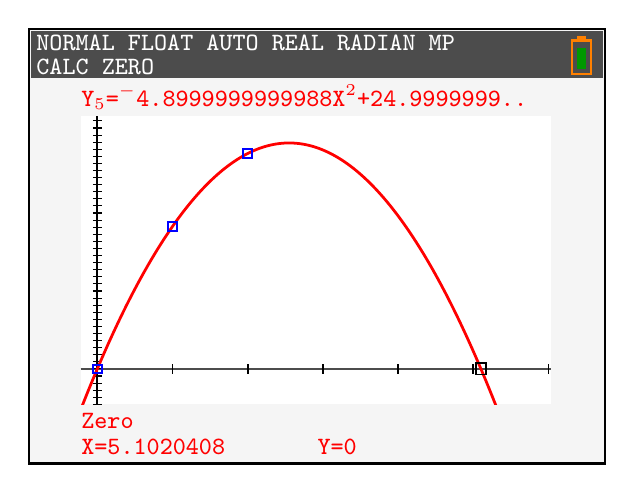
\begin{tikzpicture}[x=0.03cm, y=-0.03cm, >=stealth,
    every node/.style={inner sep=0pt, font=\small\ttfamily}]
  % TI-84 Plus CE screen, 244 x 184 px; coordinates are screen pixels
  \fill[gray!8] (0,0) rectangle (244,184);
  \draw[black, line width=0.8pt] (0,0) rectangle (244,184);
  % Status bar
  \fill[black!70] (1,1) rectangle (243,21);
  \node[white, anchor=west] at (3,6) {NORMAL FLOAT AUTO REAL RADIAN MP};
  \node[white, anchor=west] at (3,16) {CALC ZERO};
  % Battery icon
  \draw[orange, line width=0.8pt] (230,5) rectangle (238,19);
  \fill[orange] (232,3) rectangle (236,5);
  \fill[green!60!black] (232,8) rectangle (236,17);
  % Function line (equation is truncated on screen)
  \node[red, anchor=west] at (22,29)
    {Y$_5$=$^-$4.8999999999988X$^2$+24.9999999..};
  % Graph area
  \fill[white] (22,37) rectangle (221,159);
  % Graph in math coordinates: origin at pixel (29,144),
  % 31.83 px per x unit, 3 px per y unit (Xscl = Yscl = 1)
  \begin{scope}[shift={(29,144)}, x=0.955cm, y=0.09cm]
    % x-axis with ticks at 1..6
    \draw[black!70, line width=0.6pt] (-0.22,0) -- (6.03,0);
    \foreach \t in {1,...,6}
      \draw[black, line width=0.6pt] (\t,-0.7) -- (\t,0.7);
    % y-axis with ticks every 1 unit
    \draw[black, line width=0.6pt] (0,-5) -- (0,35.7);
    \foreach \t in {-5,...,35}
      \draw[black, line width=0.4pt] (-0.06,\t) -- (0.06,\t);
    % Regression curve: y = -4.9x^2 + 25x, clipped to window
    \begin{scope}
      \clip (-0.22,-5) rectangle (6.03,35.7);
      \draw[red, line width=1pt, smooth, samples=150, domain=-0.22:5.4]
        plot (\x, {-4.9*\x*\x + 25*\x});
    \end{scope}
    % Plotted data points (blue squares): L1, L2 from 14S-1 and question 1B.A.14
    \foreach \p in {(0,0), (1,20.1), (2,30.4)}
      \draw[blue, line width=0.8pt] \p
        ++(-0.06,-0.6) rectangle ++(0.12,1.2);
    % Trace cursor at the zero
    \draw[black, line width=0.6pt] (5.102,0)
      ++(-0.07,-0.8) rectangle ++(0.14,1.6);
  \end{scope}
  % Result text
  \node[red, anchor=west] at (22,166) {Zero};
  \node[red, anchor=west] at (22,177) {X=5.1020408};
  \node[red, anchor=west] at (122,177) {Y=0};
\end{tikzpicture}
\end{document}
